\section{Breadth-first Search}
\index{breadth-first search}
\index{search!breadth-first}
\index{BFS}

Breadth-first search is a method of searching an unweighted graph of nodes.
Ultimately, the search is implemented using a queue to visit nodes in the immediate neighborhood of the current node (nodes that are separated by only one edge) before branching out to explore nodes further away.
As each node is seen, it is marked as visited.
Only nodes that have not been marked as visited are added to the queue.
Using this technique, one can find the shortest path from a given node to another node.
The running time of the algorithm can be described as $O(m + n)$ for a given graph containing $m$ nodes and $n$ edges.

\begin{figure}[h]
	\centering
	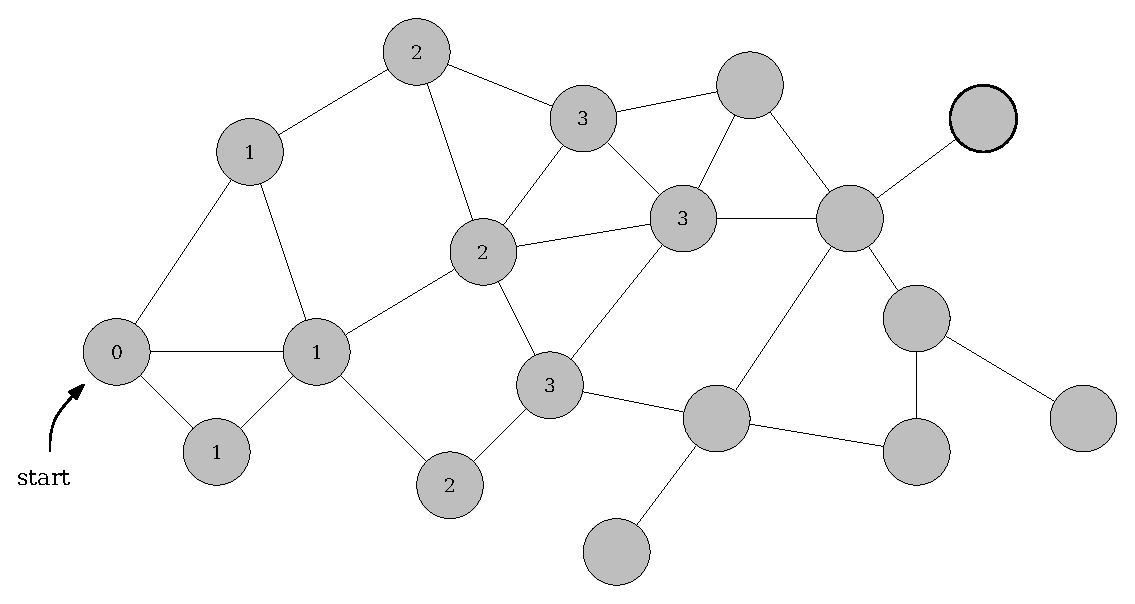
\includegraphics[width=0.6\textwidth]{./algorithms/breadth-first-search/partial-bfs}
	\caption{\small A partially completed breadth-first search on a graph with no particular target node.}
\end{figure}

\subsection{Applications}

\begin{itemize}
	\item Searching graphs with unit edges.
		Graphs with weighted edges should use the Dijkstra or Floyd-Warshall algorithm.
	\item Finding the shortest path between two given nodes.
	\item Testing a given graph for bipartiteness.
	By applying arbitrary, alternating labels to nodes as they are visited, one can determine if a graph is bipartite if a break in the alternation occurs.
\end{itemize}

\subsection{Example Contest Problem: Hopping Stones}

Contemplating wave-based trigonometric functions down by the river forming the southern edge of Farmer John's property may have kept the cows busy for a little while, but studying cowculus with their mathematics mentors is still on their mind.
They must escape the bounds of the fences.
The problem is that not all of them are able to hop the fence, and none would desire to destroy Farmer John's hard work.

There are a number of large rocks in the river that the cows could use to go around the edge of the fencing.
However, many of the cows are queasy about being over the deep waters that it holds and would rather hop around as little as possible.

Reassure the hesitating cows by finding the length of the shortest route possible for them to cross.

\subsubsection{Input}
\begin{itemize}
	\item Line 1: An unsigned integer representing the starting position of the cows.
	\item Line 2: An unsigned integer representing the number of the destination to be hopped to.
	\item Line 3 to EOF: A pair of unsigned integers representing the stones that can be hopped between.
\end{itemize}

\subsubsection{Sample Input}
\acmlisting[label=Hopping Stones Input, caption=Hopping Stones Input]{./algorithms/breadth-first-search/problems/hopping-stones/hopping-stones.in}

\subsubsection{Output}
Text formatted as in the sample output stating the number of hops that must be made to reach the specified destination.

\subsubsection{Sample Output}
\acmlisting[label=Hopping Stones Output, caption=Hopping Stones Output]{./algorithms/breadth-first-search/problems/hopping-stones/hopping-stones.out}

\subsubsection{Example Solution}
\acmlisting[label=Hopping Stones Solution, caption=Hopping Stones Solution]{./algorithms/breadth-first-search/problems/hopping-stones/hopping-stones.cpp}

\subsubsection{Lessons Learned}
\begin{itemize}
	\item If no target node is specified, the algorithm will completely propogate to all reachable nodes.
		This will result in shortest path calculation for all nodes.
	\item Representing the edges as a pair of unsigned integers is much quicker than using a dedicated struct.
\end{itemize}
